% Dynamic Follow-up Questions for Attributing Failures of RAG Chatbots
% Two-column ACL template. Compile with pdfLaTeX + BibTeX (Overleaf default).
\documentclass[11pt]{article}

% "final" shows author names. Use [review] for an anonymous version.
\usepackage[final]{acl}

\usepackage{times}
\usepackage{latexsym}
\usepackage[T1]{fontenc}
\usepackage[utf8]{inputenc}
\usepackage{microtype}
\IfFileExists{inconsolata.sty}{\usepackage{inconsolata}}{}
\usepackage{graphicx}
\usepackage{booktabs}
\usepackage{tabularx}
\usepackage{array}
\usepackage{amsmath}
\usepackage{amssymb}
\newcommand{\checkedbox}{\makebox[0pt][l]{$\square$}\raisebox{.15ex}{\hspace{0.1em}$\checkmark$}}
\usepackage{float}
\usepackage{tocloft}
\renewcommand{\contentsname}{Table of Contents}
\setlength{\cftbeforesecskip}{3pt}
\renewcommand{\cftsecleader}{\cftdotfill{\cftdotsep}}
\usepackage{enumitem}
\setlist{nosep,leftmargin=*}
\raggedbottom % stop LaTeX from stretching gaps to fill each column

\newcolumntype{L}{>{\raggedright\arraybackslash}X}

\title{Dynamic Follow-up Questions for Attributing Failures of RAG Chatbots}

\author{
  Tanyarat Suksuwan \quad Kanyanat Wasuthawat \quad Sippakorn Kanin \\
  Faculty of Information and Communication Technology, Mahidol University \\[4pt]
  \textbf{Advisors:} Asst.\ Prof.\ Dr.\ Thanapon Noraset (Mahidol University) \\
  Assoc.\ Prof.\ Dr.\ Natthawut Kertkeidkachorn (Japan Advanced Institute of Science and Technology)
}

\begin{document}

% =============================== COVER PAGE ===============================
\onecolumn
\begin{titlepage}
\centering

\includegraphics[width=0.62\textwidth]{logos.png}\par
\vspace{2cm}
{\large Internship Project Report\par}
\vspace{0.8cm}
{\LARGE\bfseries Dynamic Follow-up Questions for\\[4pt] Attributing Failures of RAG Chatbots\par}
\vspace{1.8cm}
{\large\itshape By\par}
\vspace{0.3cm}
{\large Tanyarat Suksuwan\par Kanyanat Wasuthawat\par Sippakorn Kanin\par}
\vspace{1.2cm}
{\large\itshape Advisors\par}
\vspace{0.3cm}
{\large Asst.\ Prof.\ Dr.\ Thanapon Noraset\par}
{Mahidol University\par}
\vspace{0.2cm}
{\large Assoc.\ Prof.\ Dr.\ Natthawut Kertkeidkachorn\par}
{Japan Advanced Institute of Science and Technology (JAIST)\par}
\vfill
{\large A Capstone Project Submitted in Partial Fulfillment of\\
the Requirements for\par}
\vspace{0.2cm}
{\large THE DEGREE OF BACHELOR OF SCIENCE\\
(INFORMATION AND COMMUNICATION TECHNOLOGY)\par}
\vspace{0.4cm}
{\large Faculty of Information and Communication Technology\\
Mahidol University\\
in collaboration with Japan Advanced Institute of Science and Technology\par}
\vspace{0.4cm}
{\large 2026\par}
\end{titlepage}

% ============================ TABLE OF CONTENTS ===========================
\pagenumbering{roman}
\setcounter{page}{2}
\tableofcontents
\clearpage
\pagenumbering{arabic}

% =============================== MAIN TEXT ================================
\twocolumn
\pagestyle{plain}
\maketitle
\thispagestyle{plain}

% ---------------------------------------------------------------
\addcontentsline{toc}{section}{Abstract}
\begin{abstract}
Retrieval-augmented generation (RAG) chatbots can give wrong answers for many reasons, such as missing knowledge, poor chunking, failed retrieval or weak grounding. Current evaluation methods can detect that an answer is wrong, but they cannot show which part of the RAG pipeline caused the error. They also focus mainly on single-turn questions, although real chatbots work in multi-turn conversations. In this work, we study whether dynamic follow-up questions, which are generated from how the RAG system actually answered, can attribute failures more accurately than static sub-questions. We propose a pipeline in which an LLM classifier assigns each failed turn to one of six failure types. We compare three inputs for the classifier: the failed conversation with no additional questions, the conversation with static sub-questions, and the conversation with dynamic follow-up questions. We evaluate each against human annotation using accuracy and F1 score. As a first step, we reproduce a single-turn failure classification baseline and obtain results close to the original study (39.0\% vs.\ 40.3\%). We also collect 885 failed turns from four RAG systems on the multi-turn MTRAG benchmark. A pilot annotation shows low agreement between annotators (mean Cohen's kappa 0.148), which suggests that RAG failure types are hard to separate, even for humans. These results establish the baseline and the dataset for the full comparison.
\end{abstract}

\noindent\textbf{Keywords:} retrieval-augmented generation, failure attribution, LLM-as-a-judge, question generation, multi-turn conversation

% ---------------------------------------------------------------
\section{Introduction}

\subsection{Background}
Large language models (LLMs) can answer many kinds of questions, but their knowledge is limited to their training data and they may produce statements that are not true. Retrieval-augmented generation (RAG) reduces this problem by connecting the LLM to an external knowledge base \citep{lewis2020rag}. A RAG system has two main processes. In the \textbf{indexing process}, documents are split into chunks, each chunk is converted into a vector by an embedding model, and the vectors are stored in a database. In the \textbf{query process}, the user question is converted into a vector, the most similar chunks are retrieved, and the LLM uses these chunks to generate the answer. RAG is now widely used in chatbots for customer support, finance, government services and technical documentation.

\subsection{Problem Statement}
A RAG system has many stages, and an error in the final answer can come from any of them. Current RAG evaluation can often tell \emph{that} an answer is wrong, but it does not clearly tell \emph{why} it is wrong. For example, a wrong answer may happen because:
\begin{itemize}
  \item the corpus does not contain the answer;
  \item the evidence was badly chunked;
  \item the retriever missed the correct chunk;
  \item the correct chunk was retrieved but not selected for generation; or
  \item the model answered only part of the question.
\end{itemize}
Without this information, developers do not know which component to improve. The problem is harder in multi-turn conversations, because a follow-up question often depends on earlier turns, and an error can come from the conversation history as well as from the current turn.

\subsection{Research Question and Objectives}
This project asks the following research question:
\begin{quote}
\emph{RQ: Can dynamic follow-up questions attribute failures of RAG more accurately than static sub-question generation?}
\end{quote}
The objectives of the project are:
\begin{enumerate}
  \item To develop and evaluate a \textbf{dynamic follow-up question} framework that uses runtime traces of the RAG system (the conversation log, retrieved chunks and answers) and multi-turn context.
  \item To attribute RAG pipeline failures (such as retrieval misses, context selection errors and grounding failures) more accurately than static sub-question generation methods.
  \item To build a human-annotated dataset of failure types for multi-turn RAG conversations.
\end{enumerate}

\subsection{Scope}
\begin{itemize}
  \item The project covers both single-turn and \textbf{multi-turn} RAG conversations.
  \item The method should \textbf{generalize to many datasets}, so it is tested on a development set and a held-out set from different domains.
  \item The project focuses on the \textbf{English language} only.
  \item The project attributes failures after they happen; it does not aim to repair the RAG system.
\end{itemize}

\subsection{Significance}
If dynamic follow-up questions can identify the cause of a failure more accurately, RAG developers can find and fix the weak component faster, for example by changing the chunking strategy, the retriever or the prompt. The project also contributes a failure taxonomy that is extended to multi-turn conversations and a human-annotated set of failed multi-turn turns.

\subsection{Structure of the Report}
Section~\ref{sec:related} reviews related work and states the research gap. Section~\ref{sec:method} describes the methodology. Section~\ref{sec:results} reports the initial results, and Section~\ref{sec:discussion} discusses them. Section~\ref{sec:plan} gives the timeline and plan, and Section~\ref{sec:conclusion} concludes the report.

% ---------------------------------------------------------------
\section{Related Works}
\label{sec:related}

\subsection{Overview of the Review}
We reviewed 63 papers on chatbot and RAG evaluation. The papers were recorded in a shared spreadsheet with their year, venue, link and labels (RAG-related, evaluation, LLM-as-a-judge, failure analysis, dataset). We found three main groups of related work (Table~\ref{tab:areas}). A paper can belong to more than one group.

\begin{table}[t]
\centering\small
\begin{tabularx}{\columnwidth}{@{}l r L@{}}
\toprule
\textbf{Research area} & \textbf{Papers} & \textbf{Main focus} \\
\midrule
LLM-as-a-judge & 37 & Using an LLM to score or compare answers \\
Question generation & 16 & Generating questions to test or probe a system \\
RAG failure attribution & 11 & Classifying why a RAG answer is wrong \\
\bottomrule
\end{tabularx}
\caption{Number of reviewed papers in each research area.}
\label{tab:areas}
\end{table}

\subsection{LLM-as-a-Judge}
LLM-as-a-judge means that a strong LLM is used to evaluate the output of another model, usually with a rubric and a scoring prompt. This approach is cheaper and faster than human evaluation, and several studies show that it agrees reasonably well with human preferences \citep{zheng2023judging,li2024llmsasjudges,li2025generation}. In the RAG setting, frameworks such as RAGAS \citep{es2024ragas} and ARES \citep{saadfalcon2024ares} use LLM judges to measure faithfulness, answer relevance and context relevance.

\paragraph{Single-turn and multi-turn evaluation.}
Most LLM-as-a-judge papers evaluate single-turn question answering. In our review, only \textbf{18.2\%} of the LLM-as-a-judge papers evaluate multi-turn or interactive conversations, while \textbf{81.8\%} use single-turn settings. Examples of multi-turn work include MT-Bench \citep{zheng2023judging}, MT-Bench-101 \citep{bai2024mtbench101}, RAD-Bench \citep{kuo2024radbench}, the FutureDial-RAG challenge, and simulated conversational QA with LLM-to-LLM interaction \citep{abbasiantaeb2024}. MT-Bench-101 gives the judge the full conversation context, including earlier turns, and asks it to score the latest response with a rubric. Multi-turn evaluation is important because context shifts, dependencies between turns and error propagation over time can only be observed across several turns. \citet{laban2025lost} also show that LLM performance drops clearly when a task is spread across several turns.

\paragraph{Judge criteria.}
The reviewed papers use many judge criteria. We grouped them into ten main criteria (Appendix~\ref{app:criteria}). The most common are helpfulness/relevance, factuality/faithfulness, citation support, reasoning, completeness, consistency, safety, abstention (negative rejection), robustness to judge bias, and efficiency/interpretability.

\paragraph{Summary.}
Most studies use single-turn evaluation, although most RAG chatbots are deployed in multi-turn settings. Also, judge criteria measure the correctness of the answer and its alignment with human expectations, but they do \textbf{not} attribute the root cause of a failure inside the RAG pipeline.

\subsection{Question Generation for Evaluation}

\paragraph{Types of generated questions.}
Question generation is often used to build test sets for RAG systems. The reviewed papers generate many types of questions, including fact (single-hop), multi-hop, information integration, negative rejection, noise robustness, counterfactual robustness, open-ended, multi-turn dialogue, fine-grained citation, domain-specific, knowledge-intensive and instruction-following questions (Appendix~\ref{app:qtypes}). For example, the RGB benchmark \citep{chen2024rgb} tests noise robustness, negative rejection, information integration and counterfactual robustness. However, these question types are mainly used to \textbf{evaluate} RAG performance, not to \textbf{probe} the cause of a RAG failure.

\paragraph{Methods of generating questions.}
We classified the question-generation papers by how the questions are created (Table~\ref{tab:qgen}).

\begin{table}[t]
\centering\small
\begin{tabularx}{\columnwidth}{@{}l r L@{}}
\toprule
\textbf{Method} & \textbf{Share} & \textbf{Description (examples)} \\
\midrule
Static single & 50.0\% & Questions are created once, before the system answers (RAGAS, ARES, RGB, HopWeaver) \\
Dynamic single & 28.6\% & One question is created from the system output or evidence (Self-RAG, JudgeLRM) \\
Dynamic follow-up & 21.4\% & A sequence of questions, each depending on the previous answer (LM-as-an-Examiner, RAD-Bench) \\
\bottomrule
\end{tabularx}
\caption{Methods used to generate questions in the reviewed papers.}
\label{tab:qgen}
\end{table}

\citet{xie2024subquestion} is the closest work to this project. They break a question into \textbf{core}, \textbf{background} and \textbf{follow-up} sub-questions and check whether each sub-question is covered by the retrieved chunks and by the final answer. Their sub-question coverage agrees well with human preference and helps improve LLM-as-a-judge evaluation. However, their sub-questions are \textbf{static and single-turn}: they are created from the original question only, and they are not used to classify failure types.

\citet{kim2024interviewer} propose \emph{LLM-as-an-Interviewer}, where one LLM acts as an interviewer and asks another LLM follow-up questions based on its previous answers and on its error type. This dynamic approach can reveal more about a model's understanding and reduces problems such as data contamination and verbosity bias. It was designed for math and depth-QA tasks, not for RAG failure attribution.

\paragraph{Summary.}
Many types of questions exist, but they aim to evaluate RAG, not to probe RAG failures. The literature suggests two useful ideas: probing questions should depend on the conversation (\textbf{dynamic}, not static), and asking several questions may reveal more information (\textbf{follow-up}, not single).

\subsection{RAG Failure Types}
\citet{barnett2024seven} describe seven failure points found when engineering RAG systems. RAGChecker \citep{ru2024ragchecker} gives fine-grained diagnostic metrics for the retriever and the generator. \citet{leung2025ragec} propose a taxonomy of errors across the RAG stages (chunker, retrieval, reranker and generator), annotate failed responses on the DragonBall dataset, and introduce an automatic LLM-based error classifier called RAGEC. Their study uses single-turn questions and uses only the conversation trace, with no additional probing questions.

Based on these studies, this project uses \textbf{six failure types} (Table~\ref{tab:failures}). The first four happen in the retrieval part of the pipeline, and the last two happen in the generation part. We found that these failure types can also be applied to multi-turn conversations if the definitions are extended (Appendix~\ref{app:failures}).

\begin{table}[t]
\centering\small
\begin{tabularx}{\columnwidth}{@{}l l L@{}}
\toprule
\textbf{Failure type} & \textbf{Part} & \textbf{Short definition} \\
\midrule
Knowledge Boundary & Retr. & The system does not recognize that the answer is outside the available evidence. \\
Chunking & Retr. & The information exists, but the chunk structure makes it hard to retrieve or use. \\
Retrieval & Retr. & Relevant evidence exists in the index but is not retrieved. \\
Context Selection & Retr. & Relevant evidence is retrieved but not selected for generation. \\
Grounding & Gen. & The answer is inconsistent with, not supported by, or goes beyond the evidence. \\
Response Coverage & Gen. & The answer is supported but incomplete for the user's request. \\
\bottomrule
\end{tabularx}
\caption{Six RAG failure types used in this project (Retr.\ = retrieval part; Gen.\ = generation part).}
\label{tab:failures}
\end{table}

\subsection{Research Gap}
The review shows the following gaps:
\begin{enumerate}
  \item Most work uses LLM-as-a-judge to \textbf{evaluate} RAG answers, not to \textbf{attribute} the cause of failures.
  \item A framework for failure-type classification exists, but only for \textbf{single-turn} RAG \citep{leung2025ragec}.
  \item Probing questions have been used to investigate RAG behaviour \citep{xie2024subquestion}, but they are \textbf{static} and are not conditioned on how the RAG system actually answered.
\end{enumerate}
No study has tested whether \textbf{dynamic follow-up questions} can improve the attribution of RAG failures, especially in \textbf{multi-turn} conversations. This project addresses this gap.

% ---------------------------------------------------------------
\section{Methodology}
\label{sec:method}

\begin{figure*}[t]
\centering
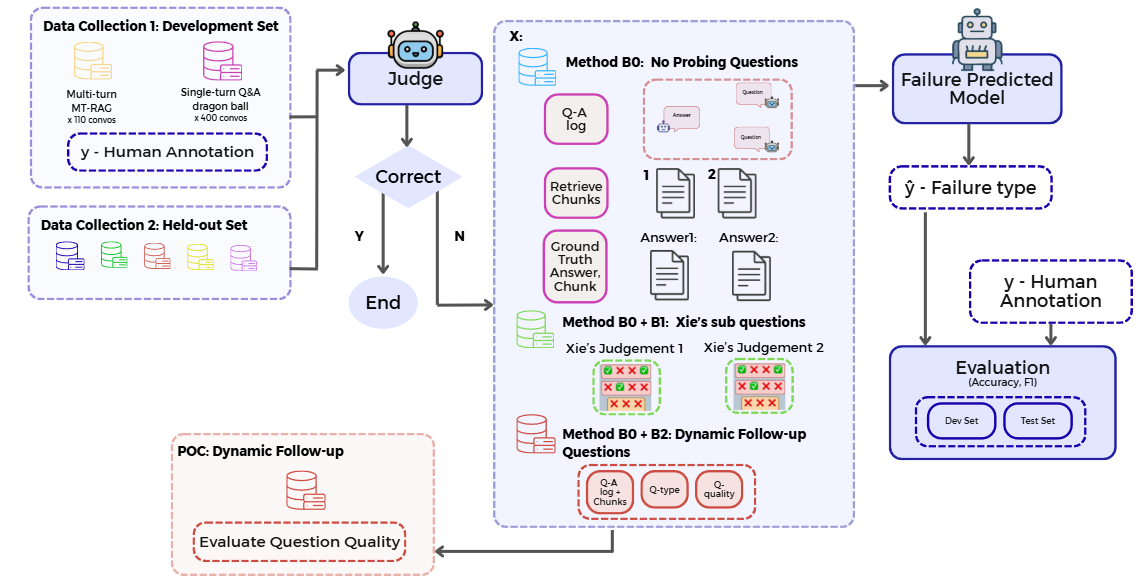
\includegraphics[width=\textwidth]{figure1.png}
\caption{Overview of the research pipeline.}
\label{fig:pipeline}
\end{figure*}

\subsection{Research Design}
This study uses an experimental design. The independent variable is the type of extra information given to a failure classifier: no probing questions (B0), static sub-questions (B1) or dynamic follow-up questions (B2). The dependent variable is how well the classifier's predicted failure type ($\hat{y}$) matches the human-annotated failure type ($y$). Figure~\ref{fig:pipeline} shows the overall pipeline.

\subsection{Data Collection}

\paragraph{Development set: DragonBall (single-turn).}
DragonBall is a single-turn question-answering dataset in finance, legal and medical domains, originally created in RAGEval \citep{zhu2024rageval} and later annotated with failure types by \citet{leung2025ragec}. It contains about 400 conversations answered by a standard RAG system (LLaMA-3 8B as the generator and GTE-Large English as the embedding model). We reproduced the retrieved chunks so that every case has the full input needed by our pipeline.

\paragraph{Development set: MTRAG (multi-turn).}
MTRAG is a human-created benchmark of multi-turn RAG conversations \citep{katsis2025mtrag}. It contains 110 conversations with an average of 7.7 turns, for 842 evaluation tasks, in four domains: CLAPnq (Wikipedia), FiQA (finance), Govt (government) and Cloud (technical documentation). MTRAG has no existing failure-type labels. We therefore ran four RAG systems on it: a standard vector RAG, RAPTOR \citep{sarthi2024raptor}, Self-RAG \citep{asai2024selfrag} and HippoRAG~2 \citep{gutierrez2025hipporag2} (Appendix~\ref{app:rag}). We then annotate the failure type of each failed turn.

\paragraph{Held-out set.}
To test generalization across domains, we will sample a small number of conversations from four to five other existing datasets, such as CORAL, MultiDoc2Dial and FinanceBench (Appendix~\ref{app:datasets}). The held-out set is not used when designing the prompts.

\subsection{Judge Step}
An LLM judge first decides whether each answer is correct by comparing it with the reference answer.
\begin{itemize}
  \item \textbf{Single-turn:} one prompt judges the question-answer log. If the answer is correct, the pipeline stops for that case. If it is incorrect, the log is sent to question generation and failure prediction.
  \item \textbf{Multi-turn:} the judge evaluates the conversation turn by turn. If all turns are correct, the pipeline stops. If any turn is incorrect, every incorrect turn is sent to the next step. Therefore one multi-turn conversation can have several failure annotations.
\end{itemize}

\subsection{Question Generation Methods}
For every failed turn, we prepare three versions of the input to the failure classifier (Table~\ref{tab:conditions}).

\begin{table*}[t]
\centering\small
\begin{tabularx}{\textwidth}{@{}p{3.2cm} p{3.4cm} L p{3.6cm}@{}}
\toprule
\textbf{Method} & \textbf{Input} & \textbf{Generation strategy} & \textbf{Output given to classifier ($X$)} \\
\midrule
B0: No additional questions & Failed Q-A log; retrieved chunks; ground-truth answer and chunk & None (no additional questions). & Q-A log + chunks + ground truth \\
B0 + B1: Static sub-questions \citep{xie2024subquestion} & Same as B0 & Split the original question into core, background and follow-up sub-questions. Check whether the retrieved text contains the facts for each sub-question, and whether the final answer includes them. & B0 + sub-question coverage of chunks + sub-question coverage of answer \\
B0 + B2: Dynamic follow-up (proposed) & Same as B0, plus the gold answer & Generate follow-up questions that depend on how the RAG system answered, and collect the RAG system's answers to them. & B0 + dynamic follow-up Q-A log \\
\bottomrule
\end{tabularx}
\caption{The three question generation conditions.}
\label{tab:conditions}
\end{table*}

\paragraph{Approach to dynamic follow-up questions.}
The dynamic follow-up method (B2) is adapted from LLM-as-an-Interviewer \citep{kim2024interviewer}. In that work, the interviewer LLM receives the question, the model's answer history and the model's error type, and then writes a follow-up question that helps to find the source of the mistake. We make two changes for the RAG setting:
\begin{itemize}
  \item Instead of giving the interviewer a known error type, we build \textbf{LLM-based signals} from the retrieved chunks, the gold chunk and the gold answer. For example, the interviewer can see whether the gold chunk was retrieved and whether the answer is consistent with the retrieved text.
  \item We use the ``MATH Fail'' prompt of \citet{kim2024interviewer} as a template and replace its four math error types with our \textbf{six RAG failure types}.
\end{itemize}
The follow-up questions are then asked to the same RAG system, and its answers are added to the conversation log. The idea is that the way the system responds to a well-chosen follow-up question gives extra evidence about where the failure happened. For example, if the system answers correctly when the question is made more specific, the original failure is more likely to be a retrieval failure than a knowledge boundary failure. A draft prompt is given in Appendix~\ref{app:prompt}.

\paragraph{Question quality check (proof of concept).}
Before the full experiment, we will run a small proof of concept to check the quality of the generated follow-up questions. We will check whether each question is relevant to the failed turn, answerable from the corpus, and different from the original question. To support this check, we will also use judge criteria from the LLM-as-a-judge literature (Appendix~\ref{app:criteria}), such as relevance, clarity and consistency.

\subsection{Failure Prediction}
The failure prediction model is a zero-shot LLM classifier. Following DragonBall \citep{leung2025ragec}, we adapt their failure-classification prompts for our six failure types.
\begin{itemize}
  \item \textbf{Input ($X$):} the failed Q-A log, retrieved chunks, ground truth, and the question generation output (B0, B1 or B2).
  \item \textbf{Output ($\hat{y}$):} one of the six failure types in Table~\ref{tab:failures}.
\end{itemize}
The same LLM and the same prompt structure are used for all three conditions, so that any difference in performance comes from the added questions.

\subsection{Human Annotation}
Human labels ($y$) are the reference for evaluation. We wrote an annotation guideline with the definition, single-turn meaning and multi-turn meaning of each failure type, and built a web tool called \emph{RAG Failure Annotation Studio}. For each failed turn, the tool shows the conversation, the retrieved documents, the documents used to generate the answer, the reference answer and the judge result. The annotator marks each failure type as \emph{Pass}, \emph{Fail} or \emph{Not applicable} and can add notes and highlight evidence.

Three annotators label the same turns separately. We then compare their labels, discuss disagreements and update the guideline until the labels are consistent. Agreement is measured with pair-wise Cohen's kappa \citep{cohen1960}:
\begin{equation}
\kappa = \frac{p_o - p_e}{1 - p_e}
\end{equation}
where $p_o$ is the observed agreement (the proportion of items where both annotators gave the same label) and $p_e$ is the agreement expected by chance (Appendix~\ref{app:kappa}).

\subsection{Evaluation Metrics}
We compare $\hat{y}$ (failure type from the classifier) with $y$ (failure type from humans) using \textbf{accuracy} and \textbf{F1 score} (macro-averaged over the six failure types). We report results separately for the development set and the held-out set, and for single-turn and multi-turn data. Finally, we compare the three conditions (B0 vs.\ B1 vs.\ B2). The research question is answered positively if B0+B2 gives higher accuracy and F1 than B0+B1.

% ---------------------------------------------------------------
\section{Initial Results}
\label{sec:results}
This section reports the preliminary results obtained so far. The main comparison of B0, B1 and B2 has not yet been run; it is planned for October to December 2026 (Section~\ref{sec:plan}).

\subsection{Findings from the Literature Review}
\begin{itemize}
  \item Among the LLM-as-a-judge papers, 18.2\% evaluate multi-turn or interactive settings and 81.8\% evaluate single-turn settings.
  \item Among the question-generation papers, 50.0\% use static single questions, 28.6\% use dynamic single questions and 21.4\% use dynamic follow-up questions.
  \item No reviewed paper uses dynamic follow-up questions to classify the failure type of a RAG system.
\end{itemize}

\subsection{Reproduction of DragonBall Failure Classification}
We reproduced the automatic error classification of \citet{leung2025ragec} on the DragonBall dataset (Table~\ref{tab:dragonball}). \citet{leung2025ragec} report 40.3\% accuracy for error type classification and 57.8\% agreement with human annotation for stage classification. Our results (39.0\% and 57.7\%) are very close to these values.

\begin{table}[t]
\centering\small
\begin{tabularx}{\columnwidth}{@{}L r r@{}}
\toprule
\textbf{Metric} & \textbf{Count} & \textbf{\%} \\
\midrule
Total cases & 377 & 100.0 \\
Judged correct & 62 & 16.4 \\
Possibly correct & 15 & 4.0 \\
Judged wrong & 300 & 79.6 \\
\midrule
Failure type accuracy$^\dagger$ & 117 / 300 & 39.0 \\
Failure stage accuracy$^\dagger$ & 173 / 300 & 57.7 \\
\bottomrule
\end{tabularx}
\caption{Results of the DragonBall reproduction. $^\dagger$Percentage of judged-wrong cases.}
\label{tab:dragonball}
\end{table}

\subsection{Failure Rates on MTRAG}
We ran four RAG systems on the MTRAG conversations and used the judge to mark each turn as correct or incorrect (Table~\ref{tab:mtrag}). The standard vector RAG used a LLaMA-based generator and the Contriever-MS MARCO dense retriever.

\begin{table}[t]
\centering\small
\begin{tabular}{@{}l l r r r@{}}
\toprule
\textbf{Dataset} & \textbf{RAG} & \textbf{Total} & \textbf{Fail} & \textbf{Rate} \\
\midrule
CLAPnq & Self-RAG & 224 & 172 & 76.8\% \\
CLAPnq & Vector & 224 & 79 & 35.3\% \\
\midrule
Cloud & HippoRAG & 205 & 120 & 58.5\% \\
Cloud & Self-RAG & 205 & 189 & 92.2\% \\
Cloud & Vector & 205 & 119 & 58.0\% \\
\midrule
FiQA & HippoRAG & 199 & 132 & 66.3\% \\
FiQA & RAPTOR & 199 & 105 & 52.8\% \\
FiQA & Self-RAG & 199 & 159 & 79.9\% \\
FiQA & Vector & 199 & 101 & 50.8\% \\
\midrule
Govt & HippoRAG & 214 & 117 & 54.7\% \\
Govt & Self-RAG & 214 & 182 & 85.0\% \\
Govt & Vector & 214 & 112 & 52.3\% \\
\bottomrule
\end{tabular}
\caption{Turns marked as incorrect on MTRAG, by dataset and RAG system.}
\label{tab:mtrag}
\end{table}

Self-RAG had the highest fail rate in every domain (76.8\% to 92.2\%). The vector RAG on CLAPnq had the lowest fail rate (35.3\%). We decided to exclude Self-RAG from the main annotation. Without Self-RAG, \textbf{885 failed turns} need annotation. The Self-RAG conversations are used to develop and test the annotation guideline.

\subsection{Pilot Annotation Agreement}
Three annotators labelled 18 failed turns from three Self-RAG conversations on CLAPnq using the B0 input. Table~\ref{tab:kappa} shows the pair-wise Cohen's kappa for each conversation. Kappa values range from 0.023 to 0.421, and the mean over all pairs and conversations is 0.148. Following the scale of \citet{landis1977}, this is \emph{slight} agreement. Annotators 2 and 3 agreed more than the other pairs.

\begin{table}[t]
\centering\small
\begin{tabular}{@{}l c c c@{}}
\toprule
\textbf{Conversation} & \textbf{A1 vs A2} & \textbf{A1 vs A3} & \textbf{A2 vs A3} \\
\midrule
1 & 0.178 & 0.172 & 0.421 \\
2 & 0.037 & 0.123 & 0.114 \\
3 & 0.023 & 0.064 & 0.201 \\
\midrule
Mean & 0.079 & 0.120 & 0.245 \\
\bottomrule
\end{tabular}
\caption{Pair-wise Cohen's kappa in the pilot annotation (A = annotator).}
\label{tab:kappa}
\end{table}

\subsection{Static Sub-Questions on a Multi-turn Conversation}
We applied the sub-question method of \citet{xie2024subquestion} to a turn from a multi-turn conversation. The question was ``who takes photos of planes in the air'', and the RAG answer was ``Aviation photographers''. The method generated \textbf{20 sub-questions}: 1 core, 10 follow-up and 9 background. The core sub-question was ``How do military photographers capture images of military aircraft in flight?''. Many sub-questions covered topics far from the user's need, such as legal considerations, drone technology and safety (Appendix~\ref{app:subq}).

% ---------------------------------------------------------------
\section{Discussion}
\label{sec:discussion}

\paragraph{Reliability of the baseline pipeline.}
Our reproduction of the DragonBall classification gives almost the same accuracy as the original study (a difference of 1.3 percentage points for failure type and 0.1 for failure stage). This shows that our data processing, retrieved chunks and prompts are close to the original setup, so B0 is a fair baseline for later comparison. The results also confirm that zero-shot failure classification is difficult: even for single-turn data, the classifier chooses the correct failure type in only about four out of ten cases. Classifying the failure \emph{stage} (retrieval or generation) is easier than classifying the exact failure \emph{type}. This supports our idea that the classifier needs more evidence, and that extra probing questions may help.

\paragraph{Failure rates in multi-turn conversations.}
The MTRAG results show that multi-turn conversations are hard for all four RAG systems: even the best case fails on about one third of turns. This agrees with \citet{katsis2025mtrag}, who report that RAG systems struggle with later turns, unanswerable questions and context-dependent questions. The very high fail rate of Self-RAG (up to 92.2\%) may be partly caused by a mismatch between its reflection-token output format and the multi-turn setting, and not only by weak retrieval or generation. Because such failures could add noise to the failure-type labels, we excluded Self-RAG from the main annotation. The high number of failures (885 turns) also means that there is enough data to compare B0, B1 and B2.

\paragraph{Low annotation agreement.}
The low kappa values in the pilot are an important finding. Possible reasons are:
\begin{itemize}
  \item \textbf{Overlapping definitions.} Some failure types are close to each other, for example Retrieval and Context Selection, or Grounding and Response Coverage. One wrong answer can also have more than one cause.
  \item \textbf{Multi-turn context.} Annotators must decide whether the error comes from the current turn or from earlier turns, which adds judgement.
  \item \textbf{Small sample.} Only 18 turns were labelled, and kappa is unstable on small samples, especially when some labels are rare.
  \item \textbf{Early guideline.} The pilot used the first version of the guideline, before any discussion between annotators.
\end{itemize}
These results show that the guideline must be refined before the main annotation. We plan to add clear decision rules (for example, check the pipeline stages in a fixed order from Knowledge Boundary to Response Coverage), add worked examples, and allow a primary and a secondary failure type. Low human agreement also sets an upper limit for any automatic classifier, so improving it is necessary for a fair evaluation.

\paragraph{Limitations of static sub-questions.}
The example in Section~\ref{sec:results} shows a weakness of static sub-questions. The method produced many sub-questions, but most were not related to the actual failure. The sub-questions are created from the question alone, before looking at how the RAG system answered, so they cannot focus on the part of the pipeline that failed. In a multi-turn conversation, they also do not consider earlier turns. Dynamic follow-up questions are designed to solve this problem, because each question depends on the RAG system's answer and on signals from the retrieved and gold evidence. Whether this leads to more accurate failure attribution will be tested in the main experiment.

\paragraph{Limitations of the study.}
\begin{itemize}
  \item The main comparison of B0, B1 and B2 has not yet been completed, so the research question cannot be answered yet.
  \item The study uses an LLM judge to decide which turns are wrong. Judge errors can add false failures or miss real ones.
  \item Dynamic follow-up questions require extra calls to the RAG system and the LLM, which increases cost and time.
  \item The study covers English only and a limited number of RAG systems and domains.
  \item Human annotation is done by three student annotators, and agreement is currently low.
\end{itemize}

% ---------------------------------------------------------------
\section{Timeline and Plan}
\label{sec:plan}
Table~\ref{tab:plan} shows the plan for the remaining work.

\begin{table}[t]
\centering\small
\begin{tabularx}{\columnwidth}{@{}l L@{}}
\toprule
\textbf{Period} & \textbf{Activity} \\
\midrule
Sep 2026 & Develop the dynamic follow-up question generation method. \\
Sep--Oct 2026 & Collect human annotation: finalize the guideline; annotate 885 failed turns from MTRAG. \\
Oct--Nov 2026 & Collect LLM failure predictions for B0, B1 and B2: single-turn DragonBall (Oct); multi-turn MTRAG and our annotated data (Nov). \\
Nov--Dec 2026 & Improve the dynamic follow-up question generation. \\
Dec 2026 & Compare and analyse the results. \\
\bottomrule
\end{tabularx}
\caption{Project timeline.}
\label{tab:plan}
\end{table}

% ---------------------------------------------------------------
\section{Conclusion}
\label{sec:conclusion}
This report presented a project on attributing the failures of RAG chatbots with dynamic follow-up questions. The review of 63 papers showed that most research uses LLM-as-a-judge to evaluate answers rather than to find the cause of failures, that most studies use single-turn settings, and that probing questions are usually static. Existing failure classification covers only single-turn RAG.

To address this gap, we designed a pipeline that compares three inputs for a zero-shot failure classifier: the failed conversation only (B0), static sub-questions (B1), and dynamic follow-up questions (B2). We defined six failure types and extended their definitions to multi-turn conversations. The initial results show that our baseline reproduces the published DragonBall results closely, that multi-turn RAG systems fail often (35.3\% to 92.2\% of turns), and that 885 failed turns from MTRAG are available for annotation. The pilot annotation showed low agreement, so the guideline must be improved before the main annotation.

In the next months, we will develop and improve the dynamic follow-up question method, complete the human annotation, collect failure predictions for B0, B1 and B2, and compare the results with accuracy and F1 score. If dynamic follow-up questions improve failure attribution, the method can help developers find and fix weak components of RAG chatbots faster, especially in real multi-turn use.

% ---------------------------------------------------------------
\addcontentsline{toc}{section}{References}
\bibliography{references}

% ---------------------------------------------------------------
\onecolumn % appendices use one column
\appendix
\addcontentsline{toc}{section}{Appendices}

\section{Full Definitions of the Six Failure Types}
\label{app:failures}

\begin{table}[H]
\centering\small
\begin{tabularx}{\textwidth}{@{}p{2.2cm} L L L@{}}
\toprule
\textbf{Failure type} & \textbf{Description} & \textbf{Single-turn} & \textbf{Multi-turn} \\
\midrule
Knowledge Boundary & The system fails to recognize that the answer is outside the available evidence scope. & The corpus does not contain enough evidence, but the system answers anyway. & The system cannot tell whether the answer should come from retrieved evidence, prior conversation, or is unsupported by both. \\
\addlinespace
Chunking & Relevant information exists in the source collection, but the chunk structure makes it hard to retrieve or use. & Needed evidence is split, incomplete, too broad, too narrow, or lacks surrounding context. & The evidence may span what the user has built up over several turns; no chunk holds a self-contained answer to the (often under-specified) follow-up question, or sub-answers across turns are scattered. \\
\addlinespace
Retrieval & The system fails to retrieve relevant evidence that exists in the indexed corpus. & A clear standalone query has relevant chunks available, but they are not retrieved. & The follow-up query is underspecified or context-dependent, causing retrieval for the wrong entity, topic or aspect. \\
\addlinespace
Context Selection & Relevant evidence is available after retrieval but is not selected for generation. & Relevant chunks are retrieved but dropped, ranked too low, or replaced by distractors. & The system fails to select the right evidence across turns, especially when the answer needs both current-turn evidence and earlier context. \\
\addlinespace
Grounding & The answer is inconsistent with, unsupported by, or overextends beyond the selected evidence. & The model fabricates, contradicts evidence, or makes claims not supported by the context. & The model contradicts retrieved evidence or the established conversation state, mixes entities across turns, or imports unsupported prior assumptions. \\
\addlinespace
Response Coverage & The answer is supported but incomplete relative to the user's request. & The answer omits part of a multi-part question, misses key evidence, or gives only a partial answer. & The answer addresses the latest turn but misses accumulated constraints, comparisons, requested scope, or unresolved pieces from earlier turns. \\
\bottomrule
\end{tabularx}
\caption{Full definitions of the six failure types for single-turn and multi-turn conversations.}
\label{tab:app-failures}
\end{table}

Table~\ref{tab:app-failures} gives the full definition of each failure type, with its meaning in single-turn and multi-turn conversations.

\section{Main Judge Criteria in LLM-as-a-Judge Studies}
\label{app:criteria}

\begin{table}[H]
\centering\small
\begin{tabularx}{\columnwidth}{@{}p{2.6cm} L@{}}
\toprule
\textbf{Criteria} & \textbf{What it measures} \\
\midrule
Helpfulness / relevance & Does the answer solve the user's question or task? \\
Factuality / faithfulness & Is the answer correct and grounded in the given context? \\
Citation / evidence support & Does it use and cite the provided evidence correctly? \\
Reasoning / logic & Can it explain steps, handle multi-hop logic and avoid weak reasoning? \\
Completeness / coverage & Does it include all important information or atomic facts? \\
Consistency / coherence & Is the answer stable, clear and not contradictory? \\
Safety / harmlessness & Does it avoid harmful, unsafe or policy-violating content? \\
Abstain / negative rejection & Can it say ``not enough information'' when needed? \\
Robustness / bias sensitivity & Is the judge resistant to position bias, verbosity, fake citations and style artifacts? \\
Efficiency / interpretability & Is the judgment transparent and not overthinking simple tasks? \\
\bottomrule
\end{tabularx}
\caption{Main judge criteria found in the review.}
\end{table}

\section{Types of Generated Questions}
\label{app:qtypes}

\begin{table}[H]
\centering\small
\begin{tabularx}{\columnwidth}{@{}p{2.6cm} L@{}}
\toprule
\textbf{Type} & \textbf{Description} \\
\midrule
Fact (single-hop) & The answer is found in exactly one sentence or document. \\
Multi-hop / cross-document & The model must connect clues spread across several documents. \\
Information integration & Separate facts from several sources are merged into one answer. \\
Negative rejection & The model should refuse when the retrieved text does not contain the answer, instead of hallucinating. \\
Noise robustness & Tests how well the model ignores irrelevant text to find the true answer. \\
Counterfactual robustness & Checks whether the model trusts wrong information in the context. \\
Open-ended & Broad questions that need long, natural-language answers. \\
Multi-turn dialogue & A back-and-forth conversation where queries change based on history. \\
Fine-grained citation & The system must show exactly which line or document it used. \\
Domain-specific & Questions on specialized, technical documents (e.g.\ medical or product QA). \\
Knowledge-intensive & Large academic datasets that test open-domain knowledge (e.g.\ KILT, SuperGLUE). \\
Instruction following & Grades how well models follow format and style constraints. \\
\bottomrule
\end{tabularx}
\caption{Types of generated questions in the literature.}
\end{table}

\section{Example of Static Sub-Questions}
\label{app:subq}
\textbf{Question:} who takes photos of planes in the air. \textbf{RAG answer:} Aviation photographers. \textbf{Number of sub-questions:} 20 (core: 1; follow-up: 10; background: 9). \textbf{Core sub-question:} How do military photographers capture images of military aircraft in flight? Examples are listed below (T = covered, F = not covered).

\begin{table}[H]
\centering\small
\begin{tabularx}{\columnwidth}{@{}c L@{}}
\toprule
& \textbf{Sub-question} \\
\midrule
T & What are the different types of aviation photography? \\
F & Who are professional aviation photographers? \\
T & What equipment is used by photographers who take photos of planes in the air? \\
T & What techniques do photographers use to capture images of planes in flight? \\
F & Are there specific companies that specialize in aerial photography of aircraft? \\
F & Do airlines employ photographers to take pictures of their aircraft? \\
T & How do military photographers capture images of military aircraft in flight? \\
F & What role do hobbyists play in aviation photography? \\
F & What are the legal considerations for taking photographs of planes in the air? \\
F & How do photographers gain access to airfields or secure areas for shooting? \\
T & What events or airshows are popular for photographing planes in the air? \\
F & How do photographers ensure safety while taking photos of planes in the air? \\
T & What are the challenges faced by photographers when shooting planes in the air? \\
F & How has drone technology impacted the photography of planes in the air? \\
\bottomrule
\end{tabularx}
\caption{Examples of static sub-questions \citep{xie2024subquestion}.}
\end{table}

\section{RAG Systems Used}
\label{app:rag}

\begin{table}[H]
\centering\small
\begin{tabularx}{\columnwidth}{@{}l L@{}}
\toprule
\textbf{RAG system} & \textbf{Main idea} \\
\midrule
Vector RAG & One-step retrieve-and-generate with a dense retriever; no reasoning step \citep{lewis2020rag}. \\
RAPTOR & Builds a tree of recursive summaries and retrieves across several levels of abstraction \citep{sarthi2024raptor}. \\
Self-RAG & Uses reflection tokens to decide when to retrieve and to critique its own output \citep{asai2024selfrag}. \\
HippoRAG 2 & Uses a knowledge graph and Personalized PageRank for multi-hop associative retrieval \citep{gutierrez2025hipporag2}. \\
\bottomrule
\end{tabularx}
\caption{RAG systems used to collect MTRAG conversations.}
\end{table}

\section{Candidate Datasets}
\label{app:datasets}

\begin{table}[H]
\centering\small
\begin{tabularx}{\columnwidth}{@{}l l L@{}}
\toprule
\textbf{Dataset} & \textbf{Task} & \textbf{Domain / notes} \\
\midrule
DragonBall & Single & Finance, legal, medical; human failure-type labels (development set). \\
MTRAG & Multi & Wikipedia, finance, government, cloud; 110 conversations, 842 tasks (development set). \\
CORAL & Multi & Open-domain; knowledge-intensive, topic shift, citation labels. \\
MultiDoc2Dial & Multi & Open-domain; dialogues grounded in multiple documents. \\
FinanceBench & Single & Finance; questions on company financial documents. \\
RAGBench & Single & Multiple domains; candidate for held-out set. \\
KILT-HotpotQA & Multi-hop & Open domain; candidate for held-out set. \\
KILT-WoW & Single & Open domain; knowledge-intensive, free-form responses. \\
\bottomrule
\end{tabularx}
\caption{Candidate datasets for the development and held-out sets.}
\end{table}

\section{Formulas for Cohen's Kappa}
\label{app:kappa}
\begin{align}
p_o &= \frac{a}{n} \\
p_e &= \sum_{l} \frac{r_l}{n} \times \frac{c_l}{n} \\
\kappa &= \frac{p_o - p_e}{1 - p_e}
\end{align}
where $a$ is the number of items where both annotators gave the same label, $r_l$ and $c_l$ are the numbers of items that the first and second annotator gave label $l$, and $n$ is the number of items. Interpretation \citep{landis1977}: below 0 = poor; 0.00--0.20 = slight; 0.21--0.40 = fair; 0.41--0.60 = moderate; 0.61--0.80 = substantial; 0.81--1.00 = almost perfect.

\section{Draft Prompt for Dynamic Follow-up Question Generation}
\label{app:prompt}
This is a working draft adapted from the ``MATH Fail'' prompt of \citet{kim2024interviewer}. It will be revised during the project.

{\small\ttfamily\raggedright
Task: You are a question generator for diagnosing a retrieval-augmented generation (RAG) chatbot. Below is a conversation in which the chatbot gave an incorrect answer, together with the retrieved chunks and diagnostic signals. Your role is to write one follow-up question that will help reveal which part of the RAG pipeline caused the failure.\par\medskip
Instructions:\par
1. Read the diagnostic signals (for example: whether the gold chunk was retrieved; whether the gold chunk was used in the answer; whether the answer is supported by the retrieved text). Do not disclose the signals or the correct answer to the chatbot.\par
2. Consider the six possible failure types: Knowledge Boundary, Chunking, Retrieval, Context Selection, Grounding, Response Coverage.\par
3. Write a follow-up question that separates the most likely failure types. For example, rephrase the question with a clearer entity to test Retrieval, ask for the source passage to test Grounding, or ask about the missing part to test Response Coverage.\par
4. The question must fit naturally in the conversation and must be answerable from the corpus if the system works correctly.\par\medskip
Input data: Conversation history: \{dialogue\_history\} | Current question: \{question\} | RAG answer: \{rag\_answer\} | Retrieved chunks: \{retrieved\_chunks\} | Gold answer (do not disclose): \{gold\_answer\} | Gold chunk (do not disclose): \{gold\_chunk\} | Diagnostic signals: \{signals\}\par\medskip
Response format (JSON): \{"target\_failure\_types": [...], "follow\_up\_question": "..."\}\par
}


% ======================= AI USAGE ACKNOWLEDGMENT =======================
\clearpage
\addcontentsline{toc}{section}{AI Usage Acknowledgment Statement}
\begin{center}
{\large\bfseries AI USAGE ACKNOWLEDGMENT STATEMENT}
\end{center}
\vspace{0.6cm}

{\linespread{1.5}\selectfont
\setlength{\parindent}{2.5em}
We acknowledge that we have utilized Generative Artificial Intelligence (Generative AI) tools (Codex, Claude, Gemini, ChatGPT) in preparing this work. The AI tools were used for the following purposes:\par}

\vspace{0.4cm}
\begin{itemize}[label={}, leftmargin=0pt, itemsep=10pt]
  \item \checkedbox\ Idea development
  \item \checkedbox\ Research assistance (e.g., literature review)
  \item \checkedbox\ Summarization and paraphrasing
  \item \checkedbox\ Draft generation
  \item \checkedbox\ Language correction, grammar checking, or translation
  \item \checkedbox\ Code editing and debugging
  \item \checkedbox\ Code generation
  \item \checkedbox\ Employing AI in the final product (e.g., generative AI API, etc.)
  \item \checkedbox\ Other (please specify): Research words writing assistance
\end{itemize}

\vspace{1cm}
\begin{flushright}
{\large
Mr.\ Sippakorn Kanin\\[8pt]
Miss Tanyarat Suksuwan\\[8pt]
Miss Kanyanat Wasuthawat\par}
\end{flushright}

\end{document}
